\section{Adaptivity}\label{sec:adaptivity}

A regular sparse grid is constructed in a way that takes a cut in a diagonal hyperplane, which means
it treats all the dimensions equally. However, there can be an important difference between the dimensions,
i.e.~one dimension might be more important than others. This can be solved by so-called dimensional adaptivity~\cite{Gerstner2003}.

\begin{figure}
    \centering
    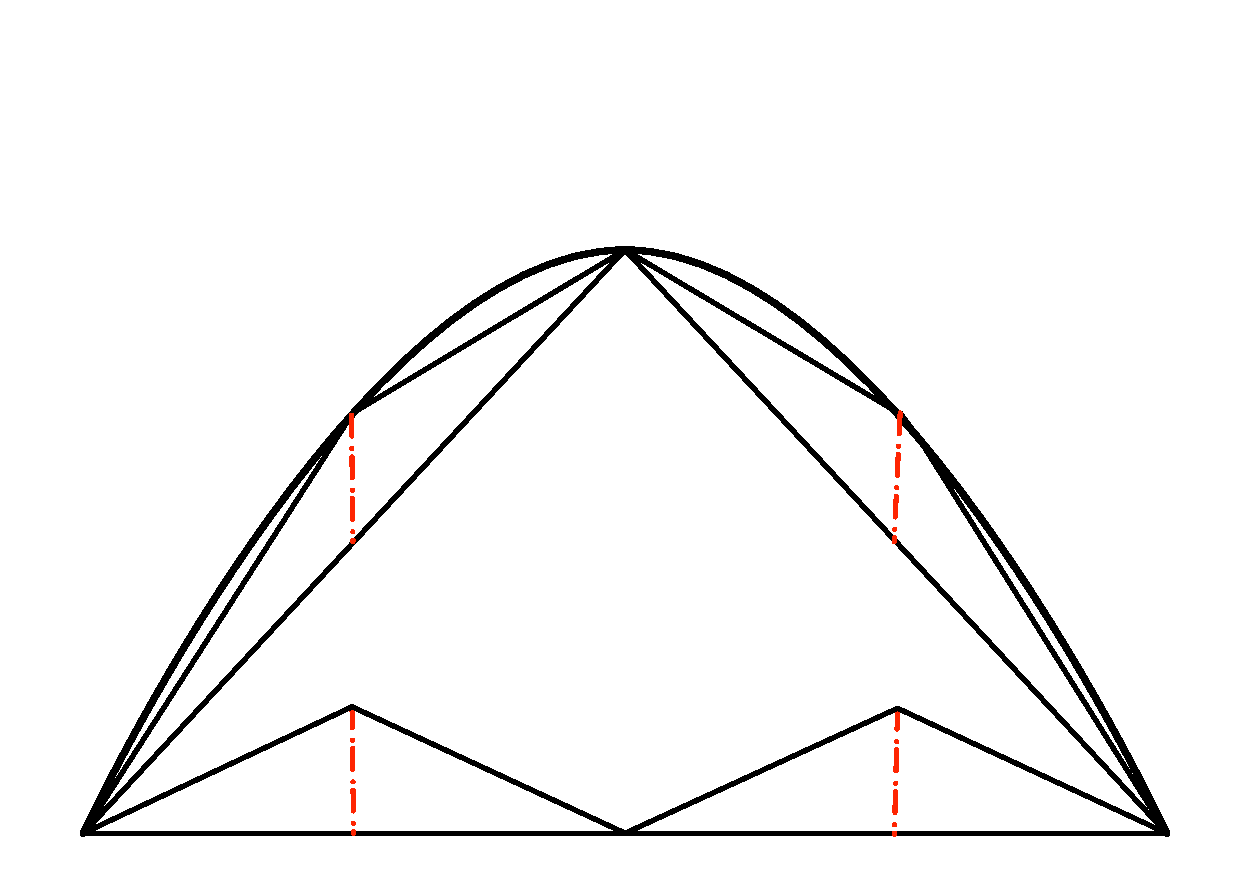
\includegraphics[keepaspectratio,height=3cm,width=0.45\textwidth]{surplus_interpolation.pdf}
    \caption{Interpolation of a parabola using 2 level hierarchical basis and surpluses, surpluses are shown in red lines.}
    \label{fig:interpolation_surplus}
\end{figure}

The most straightforward approach for this type of refinement is adding some new subspaces in the dimension in which function changes rapidly. In order to add a new subspace \(W_{\vec{l}}\), one should include all the backward neighbors in the current set of subspaces. This refinement treats all the grid points in one dimension uniformly and is called dimensionally adaptive refinement. It leads to more points in one dimension than the other one.

Moreover, some cases exist where dimensional adaptivity is insufficient to solve the problem. For instance, take a primarily flat function with peaks at specific domain regions. Franke's function~\cite{Franke1979} \cref{eqn:franke} is a good example for this, which will be used in \cref{sec:example}.

\begin{equation}
    \begin{aligned}
        f(x_1,x_2) & = \frac{3}{4} \exp \left( - \frac{(9x_1-2)^2}{4} - \frac{(9x_2-2)^2}{4} \right) \\
                   & + \frac{3}{4} \exp  \left( - \frac{(9x_1+1)}{49} - \frac{9x_2+1}{10}\right)     \\
                   & + \frac{1}{2} \exp \left( -\frac{(9x_1-7)^2}{4} - \frac{(9x_2-3)^2}{4} \right)  \\
                   & - \frac{1}{5} \exp \left( - (9x_1-4 )^2 -(9x_2-7)\right)
    \end{aligned}
    \label{eqn:franke}
\end{equation}

A dimensionally adaptive grid would also add more points to regions where the function is mostly flat.
A spatially adaptive grid~\cite{pflueger10spatially} would overcome this problem. Instead of adding whole incremental grids,
spatial adaption would only include a subset of those points near the region of interest and saves points.

The general approach for spatially adaptive grids is doing the refinement process iteratively. One could start an initial coarse grid, or one knows, a grid tailored to the problem. Using an iterative process, one could add new points (neighboring grid points in the next higher level) to the region of interest. A consistency constraint exists to enable the usage of sparse grid algorithms; the grid should contain all the hierarchical ancestors of all grid points. This may lead to the number of points added is larger than \( 2 \cdot d \) \Cref{fig:spatialrefinement} shows how this process is done in the two-dimensional regular sparse grid for one refinement step.

\begin{figure}
    \centering
    \begin{subfigure}{0.22\textwidth}
        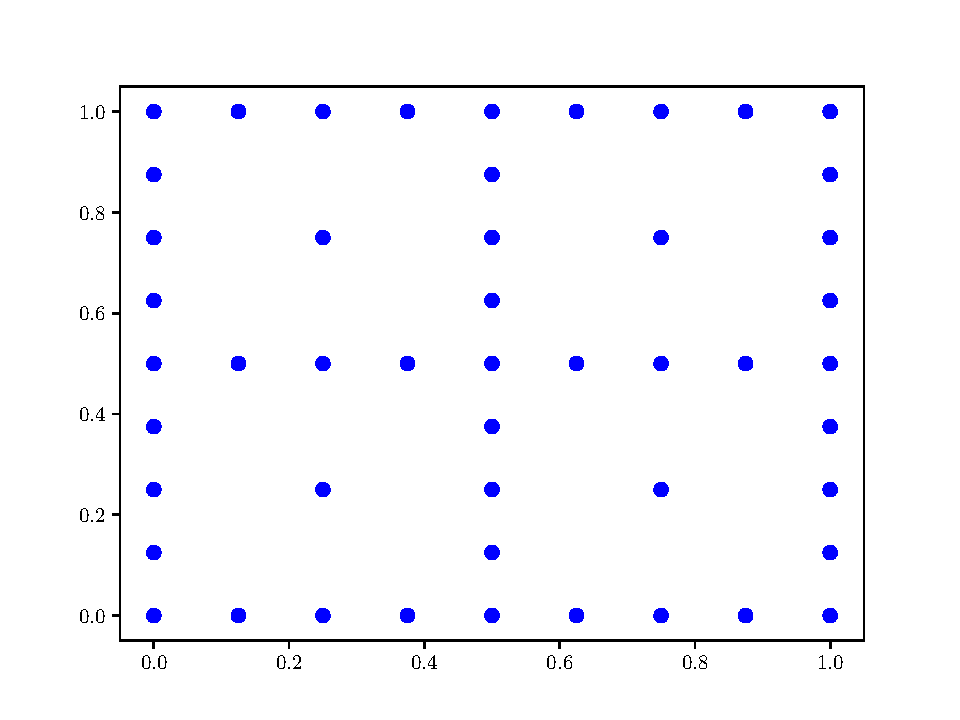
\includegraphics[width=\textwidth]{before_refinement.pdf}
        \caption{Regular grid.}
        \label{fig:regularlevel3}
    \end{subfigure}%
    \begin{subfigure}{0.22\textwidth}
        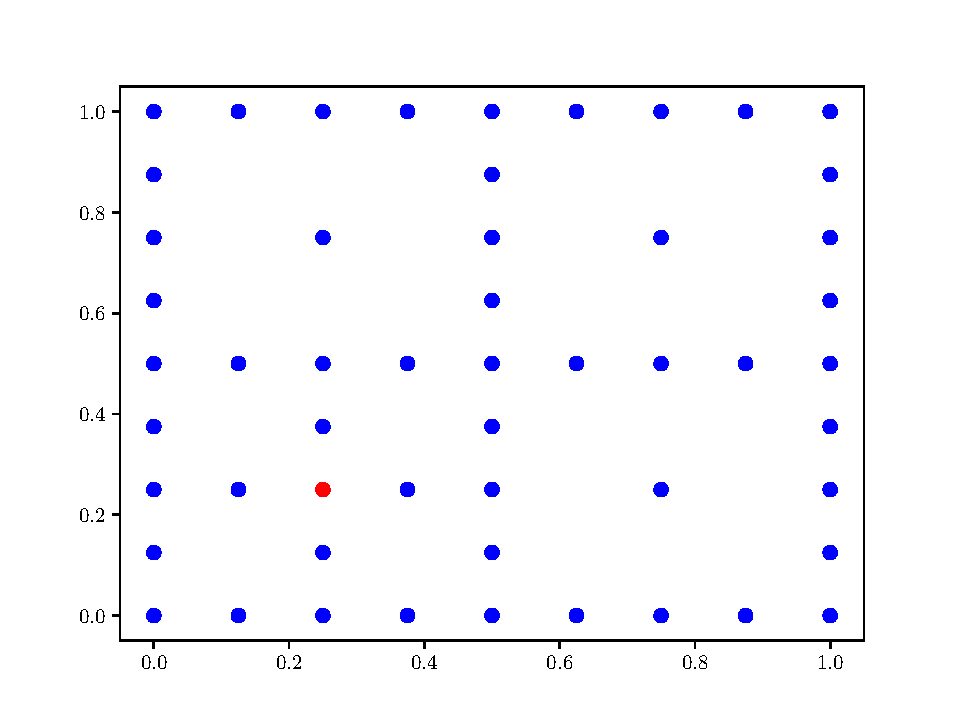
\includegraphics[width=\textwidth]{refinement_0.pdf}
        \caption{The refined grid.}
    \end{subfigure}
    \caption{Spatial refinement of a regular level 3 grid. Refinement point is marked with red.}
    \label{fig:spatialrefinement}
\end{figure}

The choice of adaptivity criteria to choose the grid points which will be refined is defined by the user. One of the most popular criteria is the surplus-based criterion, which is used in the example section in this paper. The surpluses on a parabolic equation are shown in \cref{fig:interpolation_surplus}. One can easily observe that at finer levels, surpluses are getting smaller and reduced to zero, where function has a flat behavior. This criterion uses the absolute value of the hierarchical surpluses. It is based on the assumption that a more significant absolute surplus corresponds to a larger second derivative. The choice of adaptivity criteria to choose the grid points which will be refined is defined by the user. One of the most popular criteria is the surplus-based criterion, which is used in the example section in this paper. This criterion uses the absolute value of the hierarchical surpluses. It is based on the assumption that a more significant absolute surplus corresponds to a larger second derivative.